\section{Giao diện người dùng}
Giao diện người dùng của ứng dụng webfuzzer được xây dựng dựa trên bản mẫu (template) React Reduction \parencite{react-reduction-github}. Bản mẫu này được viết trên React.js với sự hỗ trợ của thư viện Bootstrap 4, hiện thực sẵn một số thành phần như thanh điều hướng, các nút bấm, ô lựa chọn, bảng biểu, kiểu chữ,... cũng như giao diện mặc định đẹp mắt, dễ dàng chỉnh sửa theo nhu cầu lập trình. Công việc của chúng tôi là hiện thực và thiết lập luồng hoạt động của ba thành phần chính của \acrshort{ui}, đảm nhiệm được việc gọi các \acrshort{api} backend cung cấp và xử lí kết quả trả về, hiển thị được những thông tin cần thiết đồng thời đáp ứng nhu cầu kiểm thử của người dùng như yêu cầu và thiết kế \acrshort{ui} đã đề ra ở \textbf{Chương 5}.
\subsection{Trang bảng điều khiển}
% \FloatBarrier
% \begin{sidewaysfigure}[!htb]
%     \centering
%         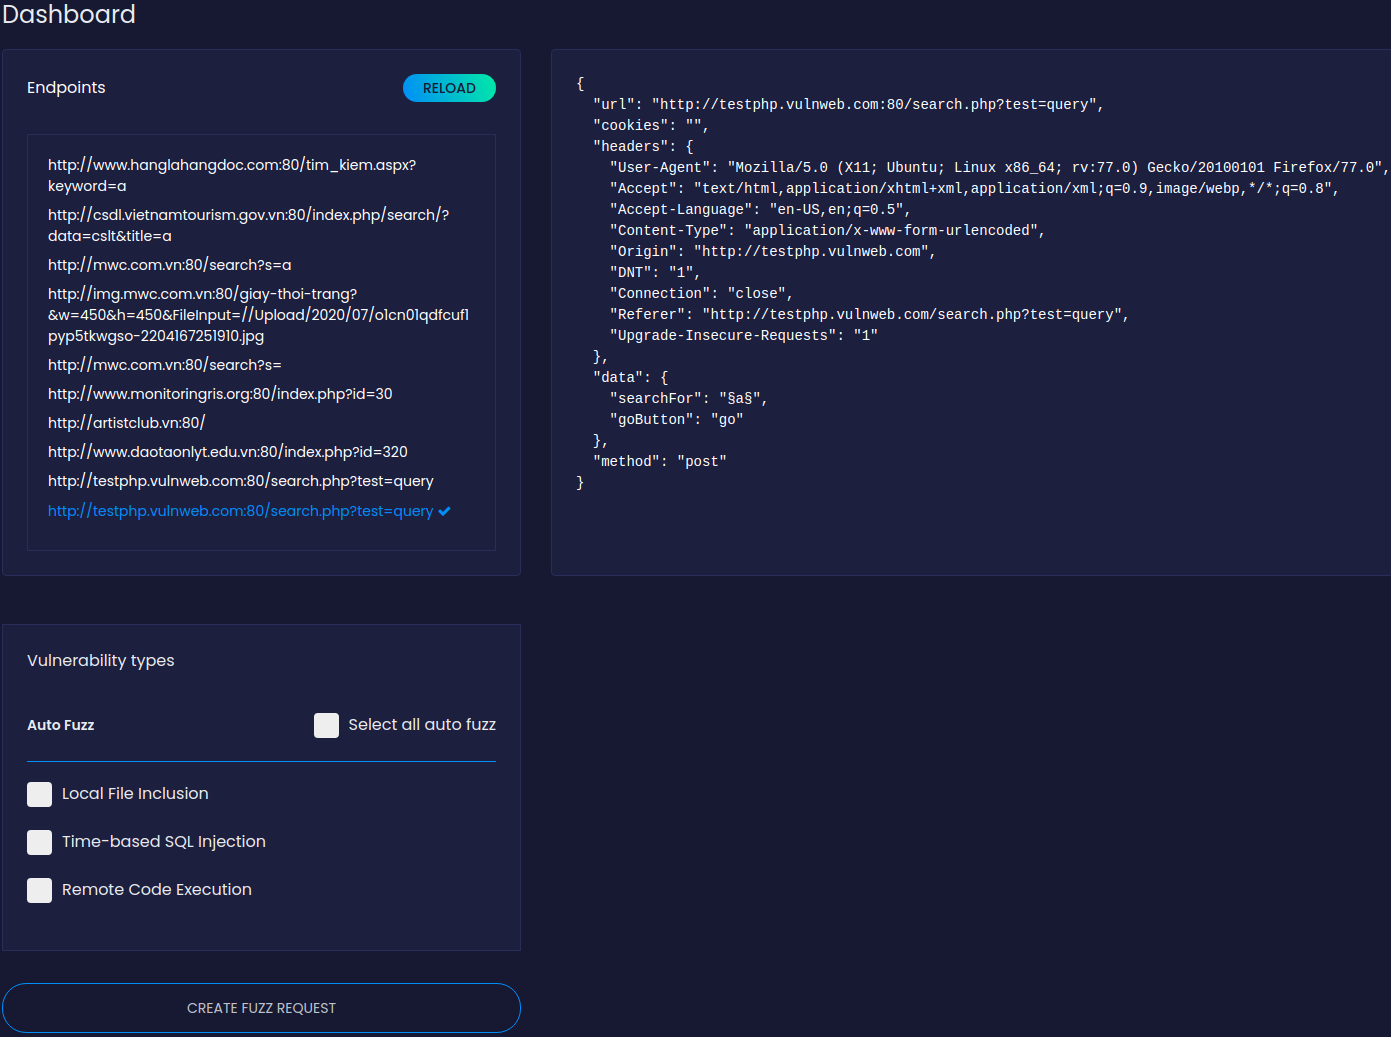
\includegraphics[scale=0.45,keepaspectratio=true]{images/dashboard-ui.png}
%     \caption{Giao diện trang bảng điều khiển ở UI ứng dụng webfuzzer}
%     \label{fig:dashboard-ui}
% \end{sidewaysfigure}
Trước tiên trong quá trình hiện thực \acrshort{ui} của ứng dụng, chúng tôi sử dụng thư viện Axios \parencite{axios-npm} để gửi \acrshort{http} request gọi \acrshort{api} tới backend ứng dụng webfuzzer. Thư viện này hỗ trợ gửi và nhận các thông điệp \acrshort{http} đơn giản thông qua việc cung cấp các tham số cần thiết như đường dẫn \acrshort{api}, phương thức \acrshort{http} kèm theo body và các tham số nếu có. Đoạn mã \ref{lst:call-API-from-UI} sau hiện thực việc gọi API và lấy ra kết quả trả về trong trường \acrshort{results} trong mã nguồn \acrshort{ui}.
\begin{lstlisting}[style=ES6, label={lst:call-API-from-UI}, caption={Gọi API từ mã nguồn UI}]
import axios from 'axios';
const BASE_URL = require('./globalConfig').BASE_URL;
const callApi = async (endpoint, method = 'get', body) => {
  try {
      let { data } = await axios({
        method: method,
        url: `${BASE_URL}${endpoint}`,
        data: body
      });
      return data.results;
  } catch (err) {
      console.log(err);
      return null;
  }
}
\end{lstlisting}
Trang này cần ba khung hiển thị thông tin 
\subsection{Trang kết quả kiểm thử}
% \FloatBarrier
% \begin{sidewaysfigure}[!htb]
%     \centering
%         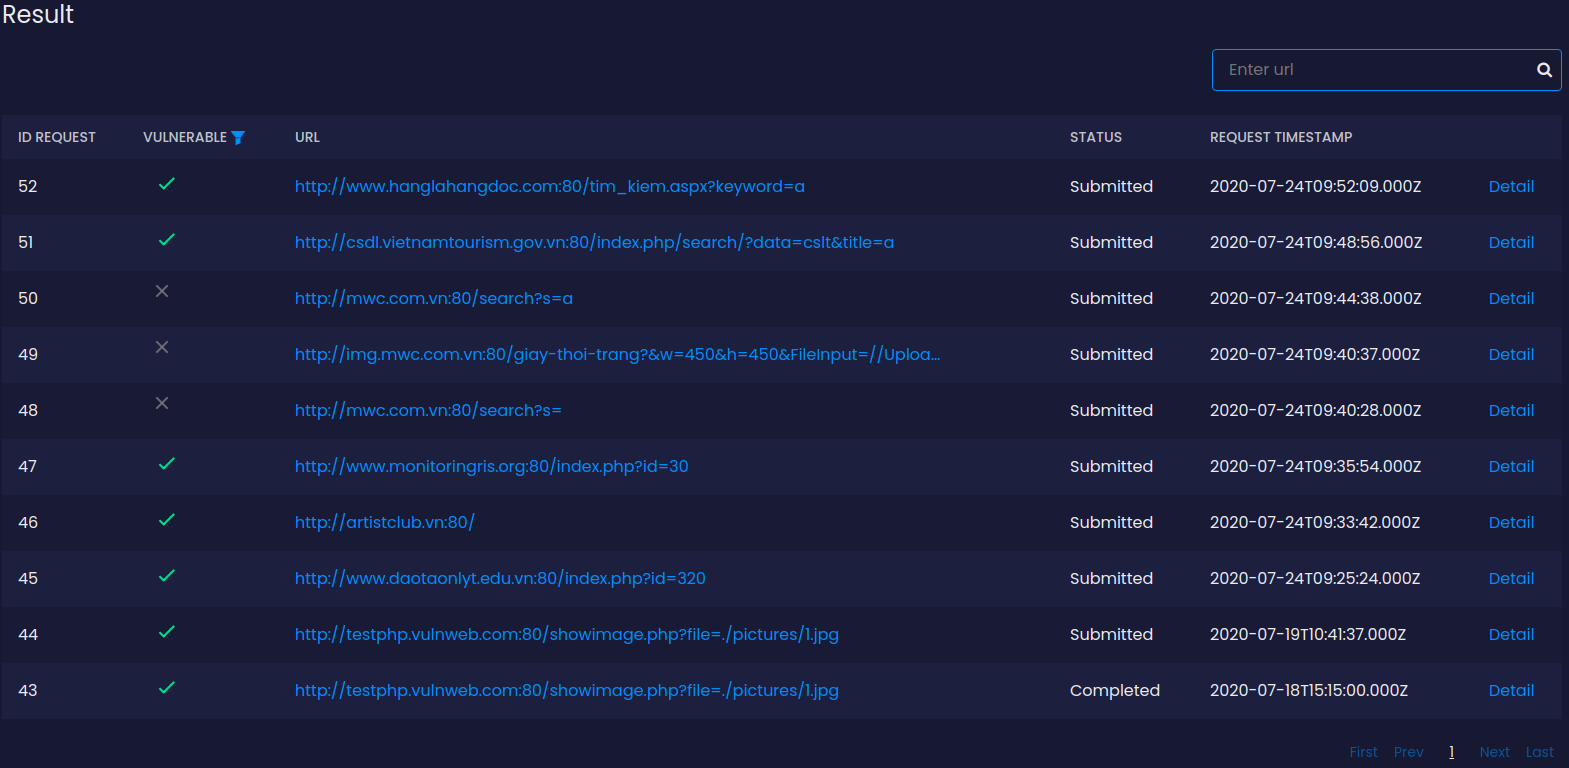
\includegraphics[scale=0.44,keepaspectratio=true]{images/result-ui.png}
%     \caption{Giao diện trang kết quả kiểm thử ở UI ứng dụng webfuzzer}
%     \label{fig:result-ui-ui}
% \end{sidewaysfigure}

\subsection{Thanh điều hướng và các thành phần khác}


\section{Cơ sở dữ liệu}
Dựa vào thiết kế đã đề ra ở \textbf{Chương 5}, chúng tôi hiện thực cấu trúc cơ sở dữ liệu của ứng dụng webfuzzer gồm ba bảng chính. Bảng \ref{tab:db-tables} dưới đây mô tả tên và chức năng của từng bảng trong lược đồ.
\begin{table}[ht]
    \centering
    \caption{Các bảng trong lược đồ quan hệ}
    \label{tab:db-tables}
    \begin{tabular}[ht]{lll}
        \toprule[1pt]\midrule[0.3pt]
            \textbf{Tên}& &\textbf{Mô tả}\\ 
        \midrule
            Endpoint& &Bảng Endpoint lưu lại các request mẫu mục tiêu được\\
            {}& &gửi đến máy chủ từ phần mở rộng Burp Suite\\
            \addlinespace
            Request& &Bảng Request lưu những yêu cầu kiểm thử một request mẫu \\
            {}& &trong bảng Endpoint của người dùng\\
            \addlinespace
            Result& &Bảng Result lưu kết quả kiểm thử chi tiết ứng với\\
            {}& &mỗi yêu cầu kiểm thử trong bảng Request\\
            \addlinespace
        \midrule[0.3pt]\bottomrule[1pt]
    \end{tabular}
\end{table}
\FloatBarrier
Hình \ref{fig:db-schema} dưới đây mô tả quan hệ giữa các bảng trong lược đồ.
\begin{figure}[H]
  \centering
    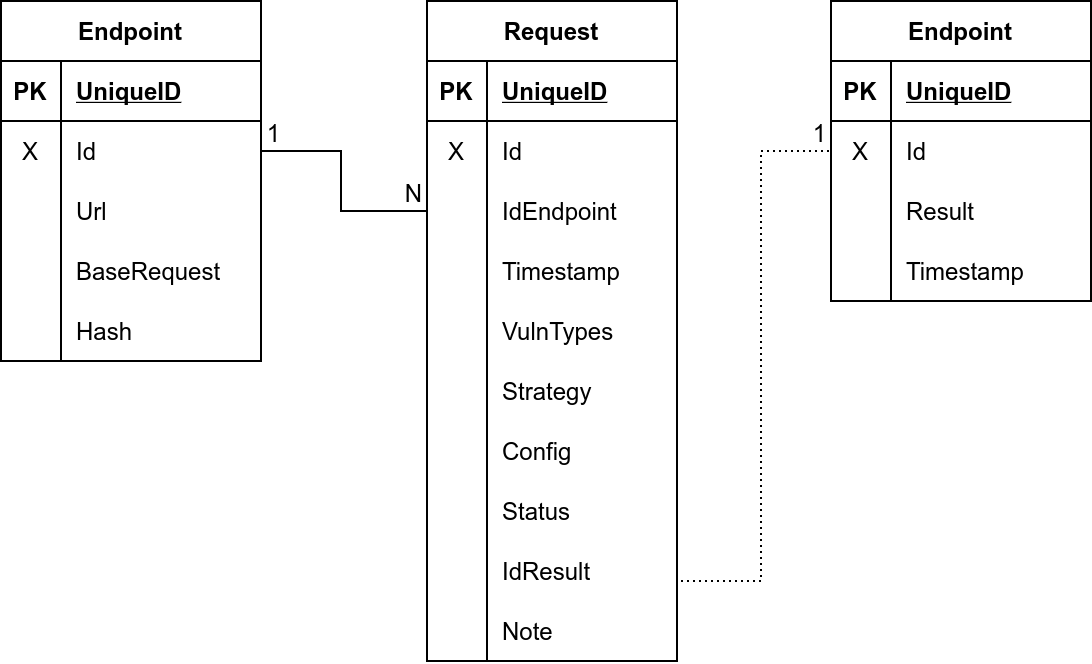
\includegraphics[width=0.75\textwidth,keepaspectratio=true]{images/database-design.png}
  \caption{Sơ đồ mối quan hệ giữa các bảng trong lược đồ}
  \label{fig:db-schema}
\end{figure}
Bảng \texttt{Endpoint} lưu trữ \acrshort{http} request mẫu được gửi từ phần mở rộng Burp Suite đến backend thông qua API \colorbox{gray!30}{\texttt{POST /}}. Request mẫu đó chứa dưới dạng chuỗi dữ liệu JSON trong trường \texttt{BaseRequest}. Trường \texttt{Url} chứa riêng \acrshort{url} của điểm cuối ứng dụng web mục tiêu để thuận lợi trong việc lọc ra những yêu cầu kiểm thử của cùng một trang web thông qua API \colorbox{gray!30}{\texttt{POST /target/search}}. Trường \texttt{Hash} chứa giá trị băm của chuỗi \texttt{BaseRequest}, đảm bảo không lưu hai request mẫu y hệt nhau gây dư thừa dữ liệu. Bảng \texttt{Request} chứa thông tin của các yêu cầu kiểm thử, trong đó trường \texttt{IdEndpoint} là khoá ngoại tham chiếu tới khoá chính \texttt{Id} của bảng \texttt{Endpoint} và trường \texttt{IdResult} là khoá ngoại tham chiếu tới khoá chính \texttt{Id} của bảng \texttt{Result} chứa kết quả kiểm thử (trong trường hợp có lỗ hổng). Mỗi bản ghi trong bảng \texttt{Request} chứa \acrshort{http} request mẫu gửi đến các điểm cuối của ứng dụng web mục tiêu, tập các lỗ hổng cần kiểm thử, trạng thái, và kết quả kiểm thử tương ứng, bao gồm danh sách lỗ hổng của điểm cuối đó và các payload phát hiện được. Trường \texttt{BaseRequest} của bảng \texttt{Endpoint}, trường \texttt{VulnTypes} của bảng \texttt{Request} và \texttt{Result} của bảng \texttt{Result} là các trường có kiểu chuỗi, chứa các giá trị kiểu đối tượng JSON đã được chuỗi hóa như đã đề cập trong phần thiết kế kiến trúc cơ sở dữ liệu ở trên.